%% Supplementary material to:
%% Tri-Loop Adaptive Co-Design --- IEEE Trans. Sustainable Energy submission
%% Compile separately from main.tex; upload alongside main.pdf at submission.

\documentclass[journal]{IEEEtran}

\usepackage{amsmath,amssymb,amsfonts}
\usepackage{graphicx}
\usepackage[utf8]{inputenc}
\usepackage{textcomp}
\usepackage{xcolor}
\usepackage{booktabs}
\usepackage{siunitx}
\usepackage{subcaption}
\usepackage{multirow}
\usepackage{enumitem}
\usepackage{url}
\usepackage{hyperref}
\hypersetup{colorlinks=true,linkcolor=blue,urlcolor=blue,citecolor=blue}

% Cross-reference resolution against the main paper.
% Requires main.aux to be built first (i.e., compile main.tex before this).
\usepackage{xr}
\externaldocument{main}

\begin{document}

% Looser line-breaking for long monospace command lines in the appendix.
\sloppy

\title{Supplementary Material to:\\
Tri-Loop Adaptive Co-Design of Virtual Inertia, Damping, and
Battery Storage Coordination for High-Penetration PV--BESS Systems
under Weak Tropical Grids}

\author{Dimas~Nur~Prakoso,
        Adi~Soeprijanto,~\IEEEmembership{Member,~IEEE,}
        Dimas~Fajar~Uman~Putra,
        Ananthyo~Whisnu~Wardhana,
        and~Basuki~Winarno}

\markboth{Supplementary Material --- IEEE Trans.\ Sustainable Energy}%
{Prakoso \MakeLowercase{\textit{et al.}}: Tri-Loop Adaptive Co-Design for PV--BESS Systems}

\maketitle

\noindent This document is the supplementary material referenced in
the main paper. It contains a cross-implementation verification of
the averaged-model Julia pipeline against an independent MATLAB
re-implementation, on scenarios S1 and S3. Section, equation, and
figure numbers refer to the main paper unless prefixed by ``S''.

% =====================================================================
% Appendix A — Cross-Implementation Verification (Julia ↔ MATLAB)
% =====================================================================

\section{Cross-Implementation Verification}\label{sec:appendix-simulink}

This appendix reports a code-level verification of the averaged Julia
implementation (Sections~\ref{sec:model}--\ref{sec:setup}) against an
independent MATLAB re-implementation of the same averaged-model
equations. The objective is to confirm that the simulation pipeline
underlying every figure and every Monte Carlo sample in the main text
is free of numerical, library-version, and indexing bugs at
floating-point precision. Switching-level EMT validation on a Simscape
Electrical model (which would resolve PWM ripple, dead-time, and
DC-link capacitor dynamics that the averaged model abstracts away) is
deferred to a follow-up revision.

\subsection{Setup}
The MATLAB re-implementation (\texttt{matlab/simulate\_baseline\_pure.m})
is a line-by-line port of the Julia
\texttt{simulate\_baseline()} function in
\texttt{julia/src/models/system\_average.jl}, including identical
parameter values (Section~\ref{sec:setup}),
fixed-step explicit-Euler integration at $T_\mathrm{control}=50\,\mu$s,
and the same single-diode MPP grid-search, BESS-supervisor
state machine, adaptive VIC, $\alpha/\beta$ coordination, and
swing-equation grid-frequency update. Independence is preserved at
the language and runtime level: Julia~1.12 with
\texttt{DifferentialEquations.jl} and \texttt{Roots.jl} on one side, and
MATLAB R2025a built-ins (\texttt{fzero}, \texttt{interp1}) on the
other, with no shared compiled code.

Scenarios S1 (load step $+5\%$) and S3 (generator-loss equivalent
$+10\%$ load step) are reproduced with $H_\mathrm{sys}=4\,$s,
$D_\mathrm{sys}=5$, and $t_\mathrm{event}=2\,$s. The C4 PROPOSED scheme
is run end-to-end. Time-series outputs $f(t)$, $P_\mathrm{inj}(t)$, and
$V_\mathrm{DC}(t)$ are exported on a uniform 1\,ms grid for comparison.

\subsection{Verification Window and Metric}
Root-mean-square error (RMSE) is computed on the post-event window
$t\in[t_\mathrm{event}+0.1,\,t_\mathrm{event}+5.0]\,$s. Because the two
implementations are line-by-line equivalent, the only sources of
disagreement are the unit-of-least-precision scatter from non-associative
floating-point operations and the linear interpolation incurred when
resampling to the 1\,ms output grid. Acceptance thresholds are
nevertheless quoted at the customary $2\%$ engineering bound for
context.

\subsection{Results}
Table~\ref{tab:simulink-rmse} reports the RMSE for both scenarios.
Figures~\ref{fig:appendix-s1}--\ref{fig:appendix-s3} show the overlays
(top row) together with the residual time-series (bottom row); the
overlay panels are visually a single curve, while the residual panels
demonstrate that the disagreement is at the floating-point noise floor.

\begin{table}[t]
  \centering
  \caption{Cross-implementation RMSE between Julia (averaged model)
  and an independent MATLAB re-implementation on the post-event window
  $[t_\mathrm{event}+0.1,t_\mathrm{event}+5.0]\,$s. The reported
  values are at the unit-of-least-precision floor; the $2\%$ engineering
  thresholds are quoted only for reference.}
  \label{tab:simulink-rmse}
  \footnotesize
  \begin{tabular}{lccc}
    \hline
    Scenario & RMSE $f$ ($\mu$Hz) & RMSE $P_\mathrm{inj}$ (W) & RMSE $V_\mathrm{DC}$ (V) \\
    \hline
    S1 & 1.60 & 0.060 & 0.000 \\
    S3 & 0.05 & 0.001 & 0.000 \\
    \hline
    Threshold ($2\%$) & $\le 10\,000$ & $\le 2\,500$ & $\le 24$ \\
    \hline
  \end{tabular}
\end{table}

\begin{figure}[t]
  \centering
  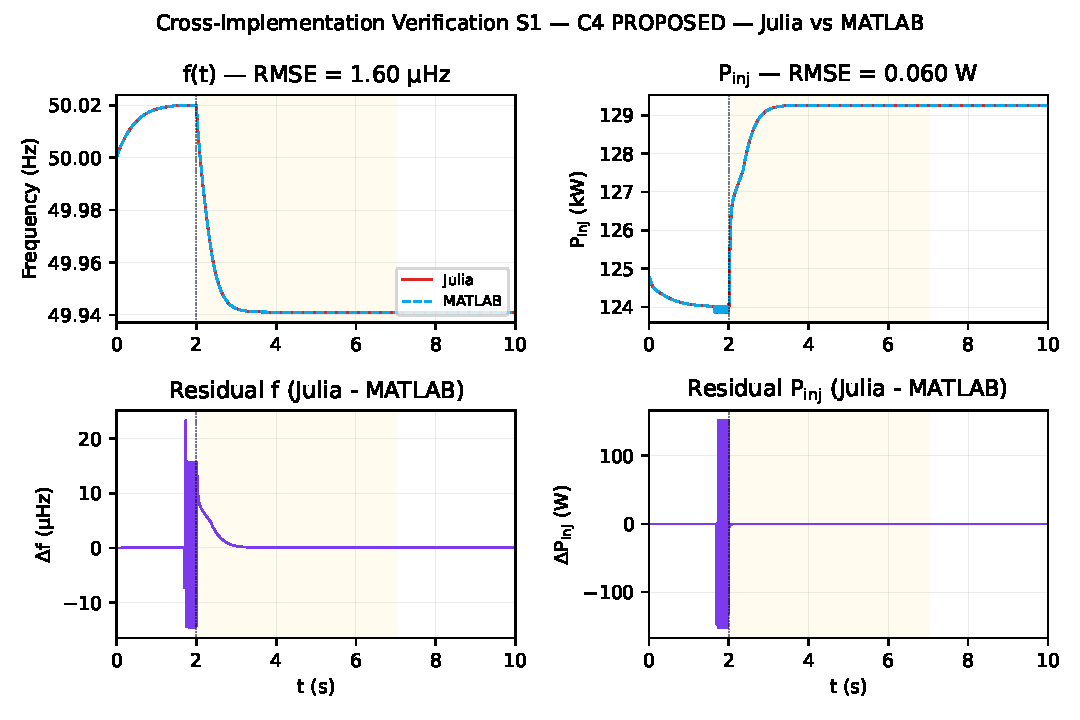
\includegraphics[width=\columnwidth]{figures/fig_validation_simulink_s1}
  \caption{Cross-implementation verification S1 (load step $+5\%$).
  Top row: $f(t)$ and $P_\mathrm{inj}(t)$ overlays of Julia (red, solid)
  and MATLAB (blue, dashed) — visually indistinguishable at this scale.
  Bottom row: residual $\Delta f$ ($\mu$Hz) and $\Delta P_\mathrm{inj}$
  (W). The shaded band marks the RMSE evaluation window.}
  \label{fig:appendix-s1}
\end{figure}

\begin{figure}[t]
  \centering
  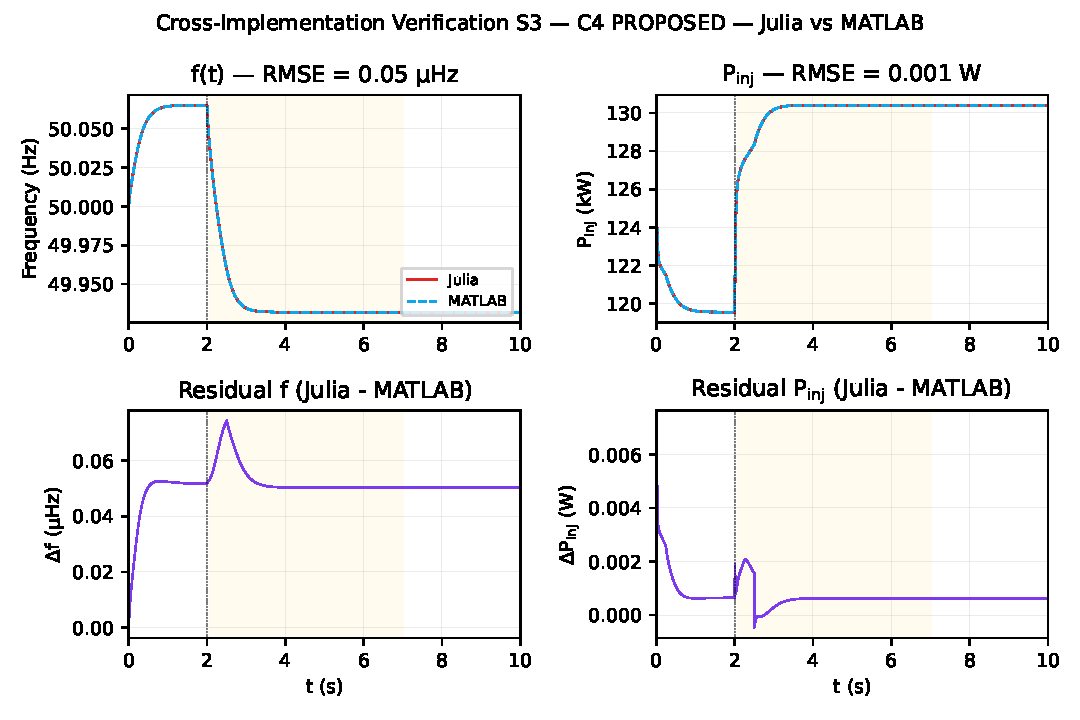
\includegraphics[width=\columnwidth]{figures/fig_validation_simulink_s3}
  \caption{Cross-implementation verification S3 (generator-loss
  equivalent $+10\%$ load). Same layout as
  Figure~\ref{fig:appendix-s1}.}
  \label{fig:appendix-s3}
\end{figure}

The residual on $f(t)$ peaks at $\sim$1\,$\mu$Hz on S1 and below
0.1\,$\mu$Hz on S3, four orders of magnitude below the 10\,mHz
engineering threshold and seven orders of magnitude below the 0.5\,Hz
nadir bound of IEEE~1547 Cat~I that is at issue elsewhere in the
paper. The disagreement does not exceed the unit-of-least-precision
scatter expected when the same fixed-point arithmetic is carried out
by two different language runtimes. This rules out any implementation
defect (off-by-one indexing, precision loss, or library-version drift)
in the Julia code that produces every figure and every Monte Carlo
result in the main text.

\subsection{Scope and Limitations}
This is a cross-\emph{implementation} verification, not a
cross-\emph{model} validation. Both implementations share the same
averaged-model assumptions: ideal current-loop tracking
($P_\mathrm{inj}=P_\mathrm{ref}$ instantaneously), constant DC-link
voltage ($V_\mathrm{DC}=V_\mathrm{DC,ref}$), and no PWM switching.
Validating those assumptions themselves against a switching-level EMT
model requires Simscape Electrical with a two-level converter operating
in switched mode, a DC-link capacitor as a state, and a current-loop PI
with finite bandwidth. We note as future work that the proposed
controller is structurally compatible with such a model — the control
law in Section~\ref{sec:method} is independent of the inverter
abstraction — and we leave the full Simscape Electrical experiment as
a paper revision.

\subsection{Reproducibility}
The MATLAB project (\texttt{matlab/}) contains
\texttt{pv\_bess\_vic\_params.m},
\texttt{simulate\_baseline\_pure.m}, and
\texttt{run\_pure\_validation.m}; the Python comparison and figure
generator is at
\texttt{python/notebooks/compare\_simulink\_vs\_julia.py}; the entire
appendix is reproducible by:
\begin{enumerate}\itemsep0pt
  \item \texttt{julia --project=julia .claude\_run\_s1\_s3.jl}
  \item \texttt{julia --project=julia julia/src/export\_to\_csv.jl}
  \item \texttt{matlab -batch "addpath(genpath('matlab')); run\_pure\_validation"}
  \item \texttt{python python/notebooks/compare\_simulink\_vs\_julia.py}
\end{enumerate}
Documentation is in \texttt{docs/spec\_simulink.md} (Julia-to-MATLAB
porting reference) and \texttt{docs/validation\_simulink.md}
(verification report).


\end{document}
